\documentclass[11pt]{amsart}

\usepackage{tikz}
\usepackage{quiver}
\usepackage{amsmath}
\usepackage{amssymb}
\usepackage{graphicx}

\title{Problems for Intro to Databases and Intro to Category Theory}

\begin{document} \maketitle

\noindent\textbf{Exercise 1.} Some exercises related to database methods.

\textbf{Part (a)} The SQL standard provides an operation \texttt{EXISTS}, which
can be used as an existential quantifier. For example,
\begin{center}
  \texttt{SELECT ... FROM ... WHERE EXISTS (<subquery>)}
\end{center}

So to express a database, we certainly need at least first-order logic. Argue
as to whether or not \textit{second}-order logic or higher is needed for any
SQL operations you are familiar with. Is first-order logic sufficient for all
SQL operations?

\textbf{Part (b)} Consider the following schema:

\begin{center}
  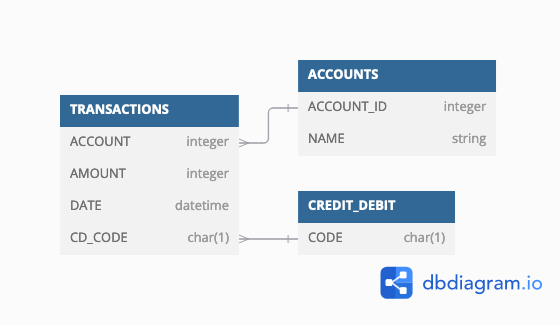
\includegraphics[width=0.5\textwidth]{schema.png}
\end{center}

Draw a diagram representing this schema, using the diagram language from the
lecture. Use filled circles for table vertices and empty circles for type
vertices.

\newpage{}

\noindent\textbf{Exercise 2.} In 1763, Leonhard Euler created a very famous
graph representing the islands of the Pregel River and the seven bridges across
it. (To understand the very simple question he wanted to solve which motivated
one of the first problems answered by graph theory, you may read the Wikipedia
article on ``The Seven Bridges of K\"onigsberg.'') Here is the graph $K$ which
he drew, with some arrows added:
\[\begin{tikzcd}
	&& B \\
	\\
	A &&&& C \\
	\\
	&& D
	\arrow["g"{description}, curve={height=-6pt}, from=1-3, to=3-1]
	\arrow["k"{description}, from=1-3, to=3-5]
	\arrow["f"{description}, curve={height=-6pt}, from=3-1, to=1-3]
	\arrow["h"{description}, from=3-1, to=3-5]
	\arrow["i"{description}, curve={height=-6pt}, from=3-1, to=5-3]
	\arrow["j"{description}, curve={height=-6pt}, from=5-3, to=3-1]
	\arrow["\ell"{description}, from=5-3, to=3-5]
\end{tikzcd}\]
Let $\mathcal{K}$ be the free category on $K$.

\bigskip

\textbf{Part (a)} List the 15 morphisms of $\mathcal{K}$ along with their
domains and codomains.

\textbf{Part (b)} A diagram is called a ``commutative'' diagram if all paths
with the same start and end point are equal; that is, if all ``parallel'' paths
through the diagram produce the same result. Let $\mathcal{K}'$ be the
\textit{commutative} free category on $K$; list the morphisms of
$\mathcal{K}'$. Using the answers of part (a) should make this a trivial
exercise.

\textbf{Part (c)} Consider the following category $\mathcal{V}$:
\[\begin{tikzcd}
  U & V & W
  \arrow["p"{description}, from=1-1, to=1-2]
  \arrow["q"{description}, from=1-3, to=1-2]
\end{tikzcd}\]
Define a functor $F : \mathcal{V} \to \mathcal{K}$.

\textbf{Pard (d)} Imagine a category that looks like this:
\[\begin{tikzcd}
	\bullet & \bullet \\
	\bullet & \bullet
	\arrow[from=1-1, to=1-2]
	\arrow[from=1-2, to=2-2]
	\arrow[from=2-1, to=1-1]
	\arrow[from=2-2, to=2-1]
\end{tikzcd}\]

Argue why there cannot be a functor from this category to $\mathcal{K}$.

\end{document}
